\documentclass[1p]{elsarticle_modified}
%\bibliographystyle{elsarticle-num}

%\usepackage[colorlinks]{hyperref}
%\usepackage{abbrmath_seonhwa} %\Abb, \Ascr, \Acal ,\Abf, \Afrak
\usepackage{amsfonts}
\usepackage{amssymb}
\usepackage{amsmath}
\usepackage{amsthm}
\usepackage{scalefnt}
\usepackage{amsbsy}
\usepackage{kotex}
\usepackage{caption}
\usepackage{subfig}
\usepackage{color}
\usepackage{graphicx}
\usepackage{xcolor} %% white, black, red, green, blue, cyan, magenta, yellow
\usepackage{float}
\usepackage{setspace}
\usepackage{hyperref}

\usepackage{tikz}
\usetikzlibrary{arrows}

\usepackage{multirow}
\usepackage{array} % fixed length table
\usepackage{hhline}

%%%%%%%%%%%%%%%%%%%%%
\makeatletter
\renewcommand*\env@matrix[1][\arraystretch]{%
	\edef\arraystretch{#1}%
	\hskip -\arraycolsep
	\let\@ifnextchar\new@ifnextchar
	\array{*\c@MaxMatrixCols c}}
\makeatother %https://tex.stackexchange.com/questions/14071/how-can-i-increase-the-line-spacing-in-a-matrix
%%%%%%%%%%%%%%%

\usepackage[normalem]{ulem}

\newcommand{\msout}[1]{\ifmmode\text{\sout{\ensuremath{#1}}}\else\sout{#1}\fi}
%SOURCE: \msout is \stkout macro in https://tex.stackexchange.com/questions/20609/strikeout-in-math-mode

\newcommand{\cancel}[1]{
	\ifmmode
	{\color{red}\msout{#1}}
	\else
	{\color{red}\sout{#1}}
	\fi
}

\newcommand{\add}[1]{
	{\color{blue}\uwave{#1}}
}

\newcommand{\replace}[2]{
	\ifmmode
	{\color{red}\msout{#1}}{\color{blue}\uwave{#2}}
	\else
	{\color{red}\sout{#1}}{\color{blue}\uwave{#2}}
	\fi
}

\newcommand{\Sol}{\mathcal{S}} %segment
\newcommand{\D}{D} %diagram
\newcommand{\A}{\mathcal{A}} %arc


%%%%%%%%%%%%%%%%%%%%%%%%%%%%%5 test

\def\sl{\operatorname{\textup{SL}}(2,\Cbb)}
\def\psl{\operatorname{\textup{PSL}}(2,\Cbb)}
\def\quan{\mkern 1mu \triangleright \mkern 1mu}

\theoremstyle{definition}
\newtheorem{thm}{Theorem}[section]
\newtheorem{prop}[thm]{Proposition}
\newtheorem{lem}[thm]{Lemma}
\newtheorem{ques}[thm]{Question}
\newtheorem{cor}[thm]{Corollary}
\newtheorem{defn}[thm]{Definition}
\newtheorem{exam}[thm]{Example}
\newtheorem{rmk}[thm]{Remark}
\newtheorem{alg}[thm]{Algorithm}

\newcommand{\I}{\sqrt{-1}}
\begin{document}

%\begin{frontmatter}
%
%\title{Boundary parabolic representations of knots up to 8 crossings}
%
%%% Group authors per affiliation:
%\author{Yunhi Cho} 
%\address{Department of Mathematics, University of Seoul, Seoul, Korea}
%\ead{yhcho@uos.ac.kr}
%
%
%\author{Seonhwa Kim} %\fnref{s_kim}}
%\address{Center for Geometry and Physics, Institute for Basic Science, Pohang, 37673, Korea}
%\ead{ryeona17@ibs.re.kr}
%
%\author{Hyuk Kim}
%\address{Department of Mathematical Sciences, Seoul National University, Seoul 08826, Korea}
%\ead{hyukkim@snu.ac.kr}
%
%\author{Seokbeom Yoon}
%\address{Department of Mathematical Sciences, Seoul National University, Seoul, 08826,  Korea}
%\ead{sbyoon15@snu.ac.kr}
%
%\begin{abstract}
%We find all boundary parabolic representation of knots up to 8 crossings.
%
%\end{abstract}
%\begin{keyword}
%    \MSC[2010] 57M25 
%\end{keyword}
%
%\end{frontmatter}

%\linenumbers
%\tableofcontents
%
\newcommand\colored[1]{\textcolor{white}{\rule[-0.35ex]{0.8em}{1.4ex}}\kern-0.8em\color{red} #1}%
%\newcommand\colored[1]{\textcolor{white}{ #1}\kern-2.17ex	\textcolor{white}{ #1}\kern-1.81ex	\textcolor{white}{ #1}\kern-2.15ex\color{red}#1	}

{\Large $\underline{12a_{0283}~(K12a_{0283})}$}

\setlength{\tabcolsep}{10pt}
\renewcommand{\arraystretch}{1.6}
\vspace{1cm}\begin{tabular}{m{100pt}>{\centering\arraybackslash}m{274pt}}
\multirow{5}{120pt}{
	\centering
	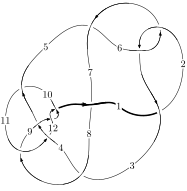
\includegraphics[width=112pt]{../../../GIT/diagram.site/Diagrams/png/1084_12a_0283.png}\\
\ \ \ A knot diagram\footnotemark}&
\allowdisplaybreaks
\textbf{Linearized knot diagam} \\
\cline{2-2}
 &
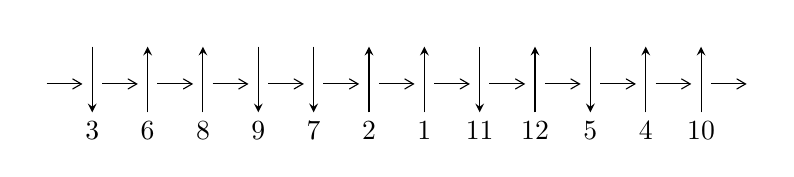
\begin{tikzpicture}[x=20pt, y=17pt]
	% nodes
	\node (C0) at (0, 0) {};
	\node (C1) at (1, 0) {};
	\node (C1U) at (1, +1) {};
	\node (C1D) at (1, -1) {3};

	\node (C2) at (2, 0) {};
	\node (C2U) at (2, +1) {};
	\node (C2D) at (2, -1) {6};

	\node (C3) at (3, 0) {};
	\node (C3U) at (3, +1) {};
	\node (C3D) at (3, -1) {8};

	\node (C4) at (4, 0) {};
	\node (C4U) at (4, +1) {};
	\node (C4D) at (4, -1) {9};

	\node (C5) at (5, 0) {};
	\node (C5U) at (5, +1) {};
	\node (C5D) at (5, -1) {7};

	\node (C6) at (6, 0) {};
	\node (C6U) at (6, +1) {};
	\node (C6D) at (6, -1) {2};

	\node (C7) at (7, 0) {};
	\node (C7U) at (7, +1) {};
	\node (C7D) at (7, -1) {1};

	\node (C8) at (8, 0) {};
	\node (C8U) at (8, +1) {};
	\node (C8D) at (8, -1) {11};

	\node (C9) at (9, 0) {};
	\node (C9U) at (9, +1) {};
	\node (C9D) at (9, -1) {12};

	\node (C10) at (10, 0) {};
	\node (C10U) at (10, +1) {};
	\node (C10D) at (10, -1) {5};

	\node (C11) at (11, 0) {};
	\node (C11U) at (11, +1) {};
	\node (C11D) at (11, -1) {4};

	\node (C12) at (12, 0) {};
	\node (C12U) at (12, +1) {};
	\node (C12D) at (12, -1) {10};
	\node (C13) at (13, 0) {};

	% arrows
	\draw[->,>={angle 60}]
	(C0) edge (C1) (C1) edge (C2) (C2) edge (C3) (C3) edge (C4) (C4) edge (C5) (C5) edge (C6) (C6) edge (C7) (C7) edge (C8) (C8) edge (C9) (C9) edge (C10) (C10) edge (C11) (C11) edge (C12) (C12) edge (C13) ;	\draw[->,>=stealth]
	(C1U) edge (C1D) (C2D) edge (C2U) (C3D) edge (C3U) (C4U) edge (C4D) (C5U) edge (C5D) (C6D) edge (C6U) (C7D) edge (C7U) (C8U) edge (C8D) (C9D) edge (C9U) (C10U) edge (C10D) (C11D) edge (C11U) (C12D) edge (C12U) ;
	\end{tikzpicture} \\
\hhline{~~} \\& 
\textbf{Solving Sequence} \\ \cline{2-2} 
 &
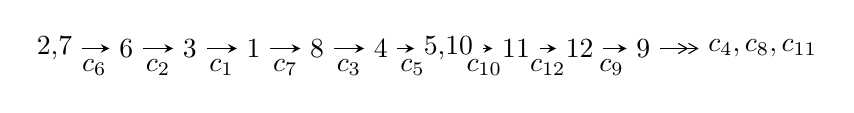
\begin{tikzpicture}[x=23pt, y=7pt]
	% node
	\node (A0) at (-1/8, 0) {2,7};
	\node (A1) at (1, 0) {6};
	\node (A2) at (2, 0) {3};
	\node (A3) at (3, 0) {1};
	\node (A4) at (4, 0) {8};
	\node (A5) at (5, 0) {4};
	\node (A6) at (97/16, 0) {5,10};
	\node (A7) at (57/8, 0) {11};
	\node (A8) at (65/8, 0) {12};
	\node (A9) at (73/8, 0) {9};
	\node (C1) at (1/2, -1) {$c_{6}$};
	\node (C2) at (3/2, -1) {$c_{2}$};
	\node (C3) at (5/2, -1) {$c_{1}$};
	\node (C4) at (7/2, -1) {$c_{7}$};
	\node (C5) at (9/2, -1) {$c_{3}$};
	\node (C6) at (11/2, -1) {$c_{5}$};
	\node (C7) at (53/8, -1) {$c_{10}$};
	\node (C8) at (61/8, -1) {$c_{12}$};
	\node (C9) at (69/8, -1) {$c_{9}$};
	\node (A10) at (11, 0) {$c_{4},c_{8},c_{11}$};

	% edge
	\draw[->,>=stealth]	
	(A0) edge (A1) (A1) edge (A2) (A2) edge (A3) (A3) edge (A4) (A4) edge (A5) (A5) edge (A6) (A6) edge (A7) (A7) edge (A8) (A8) edge (A9) ;
	\draw[->>,>={angle 60}]	
	(A9) edge (A10);
\end{tikzpicture} \\ 

\end{tabular} \\

\footnotetext{
The image of knot diagram is generated by the software ``\textbf{Draw programme}" developed by Andrew Bartholomew(\url{http://www.layer8.co.uk/maths/draw/index.htm\#Running-draw}), where we modified some parts for our purpose(\url{https://github.com/CATsTAILs/LinksPainter}).
}\phantom \\ \newline 
\centering \textbf{Ideals for irreducible components\footnotemark of $X_{\text{par}}$} 
 
\begin{align*}
I^u_{1}&=\langle 
-7.90119\times10^{36} u^{112}-1.11419\times10^{37} u^{111}+\cdots+3.32893\times10^{36} b-5.90383\times10^{36},\\
\phantom{I^u_{1}}&\phantom{= \langle  }-1.73556\times10^{37} u^{112}-1.93532\times10^{37} u^{111}+\cdots+3.32893\times10^{36} a-1.78658\times10^{37},\\
\phantom{I^u_{1}}&\phantom{= \langle  }u^{113}+2 u^{112}+\cdots+5 u+1\rangle \\
I^u_{2}&=\langle 
b+1,\;a-2 u+2,\;u^2- u+1\rangle \\
\\
\end{align*}
\raggedright * 2 irreducible components of $\dim_{\mathbb{C}}=0$, with total 115 representations.\\
\footnotetext{All coefficients of polynomials are rational numbers. But the coefficients are sometimes approximated in decimal forms when there is not enough margin.}
\newpage
\renewcommand{\arraystretch}{1}
\centering \section*{I. $I^u_{1}= \langle -7.90\times10^{36} u^{112}-1.11\times10^{37} u^{111}+\cdots+3.33\times10^{36} b-5.90\times10^{36},\;-1.74\times10^{37} u^{112}-1.94\times10^{37} u^{111}+\cdots+3.33\times10^{36} a-1.79\times10^{37},\;u^{113}+2 u^{112}+\cdots+5 u+1 \rangle$}
\flushleft \textbf{(i) Arc colorings}\\
\begin{tabular}{m{7pt} m{180pt} m{7pt} m{180pt} }
\flushright $a_{2}=$&$\begin{pmatrix}0\\u\end{pmatrix}$ \\
\flushright $a_{7}=$&$\begin{pmatrix}1\\0\end{pmatrix}$ \\
\flushright $a_{6}=$&$\begin{pmatrix}1\\u^2\end{pmatrix}$ \\
\flushright $a_{3}=$&$\begin{pmatrix}u\\u^3+u\end{pmatrix}$ \\
\flushright $a_{1}=$&$\begin{pmatrix}u^3\\u^5+u^3+u\end{pmatrix}$ \\
\flushright $a_{8}=$&$\begin{pmatrix}- u^8- u^6- u^4+1\\- u^{10}-2 u^8-3 u^6-2 u^4- u^2\end{pmatrix}$ \\
\flushright $a_{4}=$&$\begin{pmatrix}- u^{15}-2 u^{13}-4 u^{11}-4 u^9-2 u^7+2 u^3+2 u\\- u^{17}-3 u^{15}-7 u^{13}-10 u^{11}-11 u^9-8 u^7-4 u^5+u\end{pmatrix}$ \\
\flushright $a_{5}=$&$\begin{pmatrix}u^2+1\\u^2\end{pmatrix}$ \\
\flushright $a_{10}=$&$\begin{pmatrix}5.21357 u^{112}+5.81366 u^{111}+\cdots+18.2825 u+5.36683\\2.37349 u^{112}+3.34698 u^{111}+\cdots+10.5007 u+1.77349\end{pmatrix}$ \\
\flushright $a_{11}=$&$\begin{pmatrix}2.57332 u^{112}+3.57332 u^{111}+\cdots+12.2084 u+4.96666\\0.133325 u^{112}+0.0666489 u^{111}+\cdots+1.69996 u-0.0666762\end{pmatrix}$ \\
\flushright $a_{12}=$&$\begin{pmatrix}5.11321 u^{112}+5.91317 u^{111}+\cdots+17.5894 u+5.71659\\2.47326 u^{112}+3.54651 u^{111}+\cdots+11.6496 u+1.87326\end{pmatrix}$ \\
\flushright $a_{9}=$&$\begin{pmatrix}-0.233210 u^{112}-0.633170 u^{111}+\cdots-0.666853 u-1.11658\\-0.833251 u^{112}-1.66650 u^{111}+\cdots-4.04963 u-0.833250\end{pmatrix}$\\&\end{tabular}
\flushleft \textbf{(ii) Obstruction class $= -1$}\\~\\
\flushleft \textbf{(iii) Cusp Shapes $= 11.7807 u^{112}+18.4014 u^{111}+\cdots+41.3370 u+11.9807$}\\~\\
\newpage\renewcommand{\arraystretch}{1}
\flushleft \textbf{(iv) u-Polynomials at the component}\newline \\
\begin{tabular}{m{50pt}|m{274pt}}
Crossings & \hspace{64pt}u-Polynomials at each crossing \\
\hline $$\begin{aligned}c_{1},c_{5}\end{aligned}$$&$\begin{aligned}
&u^{113}+36 u^{112}+\cdots-5 u-1
\end{aligned}$\\
\hline $$\begin{aligned}c_{2},c_{6}\end{aligned}$$&$\begin{aligned}
&u^{113}-2 u^{112}+\cdots+5 u-1
\end{aligned}$\\
\hline $$\begin{aligned}c_{3}\end{aligned}$$&$\begin{aligned}
&u^{113}-34 u^{111}+\cdots-426005 u-37025
\end{aligned}$\\
\hline $$\begin{aligned}c_{4}\end{aligned}$$&$\begin{aligned}
&u^{113}+4 u^{112}+\cdots+u+1
\end{aligned}$\\
\hline $$\begin{aligned}c_{7}\end{aligned}$$&$\begin{aligned}
&u^{113}+5 u^{112}+\cdots-28640 u-6976
\end{aligned}$\\
\hline $$\begin{aligned}c_{8}\end{aligned}$$&$\begin{aligned}
&u^{113}-19 u^{112}+\cdots-12 u+4
\end{aligned}$\\
\hline $$\begin{aligned}c_{9},c_{12}\end{aligned}$$&$\begin{aligned}
&u^{113}+3 u^{112}+\cdots+2 u-1
\end{aligned}$\\
\hline $$\begin{aligned}c_{10}\end{aligned}$$&$\begin{aligned}
&u^{113}-2 u^{112}+\cdots+459991 u+41101
\end{aligned}$\\
\hline $$\begin{aligned}c_{11}\end{aligned}$$&$\begin{aligned}
&u^{113}-4 u^{112}+\cdots-58837 u+9439
\end{aligned}$\\
\hline
\end{tabular}\\~\\
\newpage\renewcommand{\arraystretch}{1}
\flushleft \textbf{(v) Riley Polynomials at the component}\newline \\
\begin{tabular}{m{50pt}|m{274pt}}
Crossings & \hspace{64pt}Riley Polynomials at each crossing \\
\hline $$\begin{aligned}c_{1},c_{5}\end{aligned}$$&$\begin{aligned}
&y^{113}+84 y^{112}+\cdots-257 y-1
\end{aligned}$\\
\hline $$\begin{aligned}c_{2},c_{6}\end{aligned}$$&$\begin{aligned}
&y^{113}+36 y^{112}+\cdots-5 y-1
\end{aligned}$\\
\hline $$\begin{aligned}c_{3}\end{aligned}$$&$\begin{aligned}
&y^{113}-68 y^{112}+\cdots+209188214975 y-1370850625
\end{aligned}$\\
\hline $$\begin{aligned}c_{4}\end{aligned}$$&$\begin{aligned}
&y^{113}+20 y^{112}+\cdots-5 y-1
\end{aligned}$\\
\hline $$\begin{aligned}c_{7}\end{aligned}$$&$\begin{aligned}
&y^{113}-17 y^{112}+\cdots-533582720 y-48664576
\end{aligned}$\\
\hline $$\begin{aligned}c_{8}\end{aligned}$$&$\begin{aligned}
&y^{113}+15 y^{112}+\cdots-280 y-16
\end{aligned}$\\
\hline $$\begin{aligned}c_{9},c_{12}\end{aligned}$$&$\begin{aligned}
&y^{113}-83 y^{112}+\cdots+26 y-1
\end{aligned}$\\
\hline $$\begin{aligned}c_{10}\end{aligned}$$&$\begin{aligned}
&y^{113}-68 y^{112}+\cdots-308333217253 y-1689292201
\end{aligned}$\\
\hline $$\begin{aligned}c_{11}\end{aligned}$$&$\begin{aligned}
&y^{113}-136 y^{112}+\cdots+1552528283 y-89094721
\end{aligned}$\\
\hline
\end{tabular}\\~\\
\newpage\flushleft \textbf{(vi) Complex Volumes and Cusp Shapes}
$$\begin{array}{c|c|c}  
\text{Solutions to }I^u_{1}& \I (\text{vol} + \sqrt{-1}CS) & \text{Cusp shape}\\
 \hline 
\begin{aligned}
u &= \phantom{-}0.189604 + 0.989106 I \\
a &= \phantom{-}0.732820 + 0.284224 I \\
b &= -1.91009 + 0.59078 I\end{aligned}
 & \phantom{-}2.22230 + 4.51942 I & \phantom{-0.000000 } 0 \\ \hline\begin{aligned}
u &= \phantom{-}0.189604 - 0.989106 I \\
a &= \phantom{-}0.732820 - 0.284224 I \\
b &= -1.91009 - 0.59078 I\end{aligned}
 & \phantom{-}2.22230 - 4.51942 I & \phantom{-0.000000 } 0 \\ \hline\begin{aligned}
u &= \phantom{-}0.026076 + 1.011230 I \\
a &= -0.862472 - 0.519253 I \\
b &= \phantom{-}1.60460 + 0.26158 I\end{aligned}
 & -5.26942 - 0.99049 I & \phantom{-0.000000 } 0 \\ \hline\begin{aligned}
u &= \phantom{-}0.026076 - 1.011230 I \\
a &= -0.862472 + 0.519253 I \\
b &= \phantom{-}1.60460 - 0.26158 I\end{aligned}
 & -5.26942 + 0.99049 I & \phantom{-0.000000 } 0 \\ \hline\begin{aligned}
u &= -0.144566 + 1.004840 I \\
a &= -0.170892 - 0.681801 I \\
b &= \phantom{-}0.398767 + 0.551773 I\end{aligned}
 & -1.95648 - 2.79535 I & \phantom{-0.000000 } 0 \\ \hline\begin{aligned}
u &= -0.144566 - 1.004840 I \\
a &= -0.170892 + 0.681801 I \\
b &= \phantom{-}0.398767 - 0.551773 I\end{aligned}
 & -1.95648 + 2.79535 I & \phantom{-0.000000 } 0 \\ \hline\begin{aligned}
u &= -0.161120 + 0.967489 I \\
a &= -2.92000 + 2.19375 I \\
b &= \phantom{-}3.14464 - 1.06906 I\end{aligned}
 & \phantom{-}0.16594 - 2.30056 I & \phantom{-0.000000 } 0 \\ \hline\begin{aligned}
u &= -0.161120 - 0.967489 I \\
a &= -2.92000 - 2.19375 I \\
b &= \phantom{-}3.14464 + 1.06906 I\end{aligned}
 & \phantom{-}0.16594 + 2.30056 I & \phantom{-0.000000 } 0 \\ \hline\begin{aligned}
u &= -0.675887 + 0.690929 I \\
a &= \phantom{-}1.48016 - 0.54011 I \\
b &= \phantom{-}0.786677 - 0.431007 I\end{aligned}
 & -0.242700 - 0.820844 I & \phantom{-0.000000 } 0 \\ \hline\begin{aligned}
u &= -0.675887 - 0.690929 I \\
a &= \phantom{-}1.48016 + 0.54011 I \\
b &= \phantom{-}0.786677 + 0.431007 I\end{aligned}
 & -0.242700 + 0.820844 I & \phantom{-0.000000 } 0\\
 \hline 
 \end{array}$$\newpage$$\begin{array}{c|c|c}  
\text{Solutions to }I^u_{1}& \I (\text{vol} + \sqrt{-1}CS) & \text{Cusp shape}\\
 \hline 
\begin{aligned}
u &= \phantom{-}0.662797 + 0.797671 I \\
a &= \phantom{-}0.33518 + 2.73691 I \\
b &= -1.26294 + 1.81134 I\end{aligned}
 & \phantom{-}3.48900 - 0.36060 I & \phantom{-0.000000 } 0 \\ \hline\begin{aligned}
u &= \phantom{-}0.662797 - 0.797671 I \\
a &= \phantom{-}0.33518 - 2.73691 I \\
b &= -1.26294 - 1.81134 I\end{aligned}
 & \phantom{-}3.48900 + 0.36060 I & \phantom{-0.000000 } 0 \\ \hline\begin{aligned}
u &= \phantom{-}0.170034 + 1.023370 I \\
a &= \phantom{-}0.576812 - 0.188643 I \\
b &= -1.44988 - 0.25305 I\end{aligned}
 & -2.23668 + 7.07465 I & \phantom{-0.000000 } 0 \\ \hline\begin{aligned}
u &= \phantom{-}0.170034 - 1.023370 I \\
a &= \phantom{-}0.576812 + 0.188643 I \\
b &= -1.44988 + 0.25305 I\end{aligned}
 & -2.23668 - 7.07465 I & \phantom{-0.000000 } 0 \\ \hline\begin{aligned}
u &= \phantom{-}0.205935 + 0.940229 I \\
a &= \phantom{-}0.083619 + 1.367930 I \\
b &= -0.599757 + 0.498152 I\end{aligned}
 & \phantom{-}2.58224 + 0.70114 I & \phantom{-0.000000 } 0 \\ \hline\begin{aligned}
u &= \phantom{-}0.205935 - 0.940229 I \\
a &= \phantom{-}0.083619 - 1.367930 I \\
b &= -0.599757 - 0.498152 I\end{aligned}
 & \phantom{-}2.58224 - 0.70114 I & \phantom{-0.000000 } 0 \\ \hline\begin{aligned}
u &= \phantom{-}0.375783 + 0.967245 I \\
a &= \phantom{-}0.50682 - 1.95144 I \\
b &= \phantom{-}0.852029 + 0.071099 I\end{aligned}
 & \phantom{-}3.49202 - 6.70621 I & \phantom{-0.000000 } 0 \\ \hline\begin{aligned}
u &= \phantom{-}0.375783 - 0.967245 I \\
a &= \phantom{-}0.50682 + 1.95144 I \\
b &= \phantom{-}0.852029 - 0.071099 I\end{aligned}
 & \phantom{-}3.49202 + 6.70621 I & \phantom{-0.000000 } 0 \\ \hline\begin{aligned}
u &= -0.630738 + 0.848947 I \\
a &= -1.42954 + 4.92205 I \\
b &= \phantom{-}1.23780 + 2.16333 I\end{aligned}
 & \phantom{-}2.25355 - 2.08148 I & \phantom{-0.000000 } 0 \\ \hline\begin{aligned}
u &= -0.630738 - 0.848947 I \\
a &= -1.42954 - 4.92205 I \\
b &= \phantom{-}1.23780 - 2.16333 I\end{aligned}
 & \phantom{-}2.25355 + 2.08148 I & \phantom{-0.000000 } 0\\
 \hline 
 \end{array}$$\newpage$$\begin{array}{c|c|c}  
\text{Solutions to }I^u_{1}& \I (\text{vol} + \sqrt{-1}CS) & \text{Cusp shape}\\
 \hline 
\begin{aligned}
u &= -0.586086 + 0.884873 I \\
a &= \phantom{-}0.496140 + 0.240299 I \\
b &= \phantom{-}0.0768557 + 0.0195798 I\end{aligned}
 & \phantom{-}0.18011 - 2.30125 I & \phantom{-0.000000 } 0 \\ \hline\begin{aligned}
u &= -0.586086 - 0.884873 I \\
a &= \phantom{-}0.496140 - 0.240299 I \\
b &= \phantom{-}0.0768557 - 0.0195798 I\end{aligned}
 & \phantom{-}0.18011 + 2.30125 I & \phantom{-0.000000 } 0 \\ \hline\begin{aligned}
u &= -0.026671 + 1.069690 I \\
a &= \phantom{-}0.529521 + 0.341317 I \\
b &= -0.90525 - 1.22531 I\end{aligned}
 & -2.88023 - 5.15805 I & \phantom{-0.000000 } 0 \\ \hline\begin{aligned}
u &= -0.026671 - 1.069690 I \\
a &= \phantom{-}0.529521 - 0.341317 I \\
b &= -0.90525 + 1.22531 I\end{aligned}
 & -2.88023 + 5.15805 I & \phantom{-0.000000 } 0 \\ \hline\begin{aligned}
u &= \phantom{-}0.186610 + 1.057550 I \\
a &= -1.166760 + 0.054768 I \\
b &= \phantom{-}1.97199 - 0.92146 I\end{aligned}
 & \phantom{-}2.31195 + 12.95770 I & \phantom{-0.000000 } 0 \\ \hline\begin{aligned}
u &= \phantom{-}0.186610 - 1.057550 I \\
a &= -1.166760 - 0.054768 I \\
b &= \phantom{-}1.97199 + 0.92146 I\end{aligned}
 & \phantom{-}2.31195 - 12.95770 I & \phantom{-0.000000 } 0 \\ \hline\begin{aligned}
u &= \phantom{-}0.804411 + 0.716895 I \\
a &= \phantom{-}0.735745 + 0.907695 I \\
b &= \phantom{-}0.33930 + 1.41948 I\end{aligned}
 & \phantom{-}4.35773 - 2.32723 I & \phantom{-0.000000 } 0 \\ \hline\begin{aligned}
u &= \phantom{-}0.804411 - 0.716895 I \\
a &= \phantom{-}0.735745 - 0.907695 I \\
b &= \phantom{-}0.33930 - 1.41948 I\end{aligned}
 & \phantom{-}4.35773 + 2.32723 I & \phantom{-0.000000 } 0 \\ \hline\begin{aligned}
u &= -0.102129 + 0.914705 I \\
a &= \phantom{-}1.154070 - 0.332979 I \\
b &= -0.843195 + 1.117950 I\end{aligned}
 & -0.90049 - 1.52806 I & \phantom{-0.000000 } 0 \\ \hline\begin{aligned}
u &= -0.102129 - 0.914705 I \\
a &= \phantom{-}1.154070 + 0.332979 I \\
b &= -0.843195 - 1.117950 I\end{aligned}
 & -0.90049 + 1.52806 I & \phantom{-0.000000 } 0\\
 \hline 
 \end{array}$$\newpage$$\begin{array}{c|c|c}  
\text{Solutions to }I^u_{1}& \I (\text{vol} + \sqrt{-1}CS) & \text{Cusp shape}\\
 \hline 
\begin{aligned}
u &= -0.819096 + 0.714745 I \\
a &= -2.15580 - 0.09456 I \\
b &= -1.93234 + 1.04877 I\end{aligned}
 & \phantom{-}4.33771 + 6.65572 I & \phantom{-0.000000 } 0 \\ \hline\begin{aligned}
u &= -0.819096 - 0.714745 I \\
a &= -2.15580 + 0.09456 I \\
b &= -1.93234 - 1.04877 I\end{aligned}
 & \phantom{-}4.33771 - 6.65572 I & \phantom{-0.000000 } 0 \\ \hline\begin{aligned}
u &= \phantom{-}0.804336 + 0.735844 I \\
a &= \phantom{-}3.49496 - 0.99406 I \\
b &= \phantom{-}3.91616 - 0.62862 I\end{aligned}
 & \phantom{-}6.48008 - 1.48579 I & \phantom{-0.000000 } 0 \\ \hline\begin{aligned}
u &= \phantom{-}0.804336 - 0.735844 I \\
a &= \phantom{-}3.49496 + 0.99406 I \\
b &= \phantom{-}3.91616 + 0.62862 I\end{aligned}
 & \phantom{-}6.48008 + 1.48579 I & \phantom{-0.000000 } 0 \\ \hline\begin{aligned}
u &= \phantom{-}0.789668 + 0.751601 I \\
a &= -1.54050 + 0.39634 I \\
b &= -1.88394 - 0.46765 I\end{aligned}
 & \phantom{-}4.99982 - 0.39403 I & \phantom{-0.000000 } 0 \\ \hline\begin{aligned}
u &= \phantom{-}0.789668 - 0.751601 I \\
a &= -1.54050 - 0.39634 I \\
b &= -1.88394 + 0.46765 I\end{aligned}
 & \phantom{-}4.99982 + 0.39403 I & \phantom{-0.000000 } 0 \\ \hline\begin{aligned}
u &= -0.401772 + 1.017800 I \\
a &= -0.591734 - 0.890779 I \\
b &= -0.716621 + 0.195724 I\end{aligned}
 & \phantom{-}2.46164 - 2.16481 I & \phantom{-0.000000 } 0 \\ \hline\begin{aligned}
u &= -0.401772 - 1.017800 I \\
a &= -0.591734 + 0.890779 I \\
b &= -0.716621 - 0.195724 I\end{aligned}
 & \phantom{-}2.46164 + 2.16481 I & \phantom{-0.000000 } 0 \\ \hline\begin{aligned}
u &= -0.198122 + 1.076290 I \\
a &= \phantom{-}0.611926 - 0.129141 I \\
b &= -1.114960 - 0.661410 I\end{aligned}
 & \phantom{-}1.26696 - 4.49664 I & \phantom{-0.000000 } 0 \\ \hline\begin{aligned}
u &= -0.198122 - 1.076290 I \\
a &= \phantom{-}0.611926 + 0.129141 I \\
b &= -1.114960 + 0.661410 I\end{aligned}
 & \phantom{-}1.26696 + 4.49664 I & \phantom{-0.000000 } 0\\
 \hline 
 \end{array}$$\newpage$$\begin{array}{c|c|c}  
\text{Solutions to }I^u_{1}& \I (\text{vol} + \sqrt{-1}CS) & \text{Cusp shape}\\
 \hline 
\begin{aligned}
u &= -0.839364 + 0.705527 I \\
a &= \phantom{-}2.43675 - 1.34274 I \\
b &= \phantom{-}1.90827 - 1.96991 I\end{aligned}
 & \phantom{-}9.1807 + 12.7383 I & \phantom{-0.000000 } 0 \\ \hline\begin{aligned}
u &= -0.839364 - 0.705527 I \\
a &= \phantom{-}2.43675 + 1.34274 I \\
b &= \phantom{-}1.90827 + 1.96991 I\end{aligned}
 & \phantom{-}9.1807 - 12.7383 I & \phantom{-0.000000 } 0 \\ \hline\begin{aligned}
u &= -0.817248 + 0.732933 I \\
a &= -2.47219 + 1.33611 I \\
b &= -1.43792 + 1.92631 I\end{aligned}
 & \phantom{-}8.80037 + 3.76825 I & \phantom{-0.000000 } 0 \\ \hline\begin{aligned}
u &= -0.817248 - 0.732933 I \\
a &= -2.47219 - 1.33611 I \\
b &= -1.43792 - 1.92631 I\end{aligned}
 & \phantom{-}8.80037 - 3.76825 I & \phantom{-0.000000 } 0 \\ \hline\begin{aligned}
u &= \phantom{-}0.701871 + 0.564677 I \\
a &= -0.49909 - 1.83088 I \\
b &= -0.249255 - 1.199190 I\end{aligned}
 & \phantom{-}2.51246 - 6.05594 I & \phantom{-0.000000 } 0 \\ \hline\begin{aligned}
u &= \phantom{-}0.701871 - 0.564677 I \\
a &= -0.49909 + 1.83088 I \\
b &= -0.249255 + 1.199190 I\end{aligned}
 & \phantom{-}2.51246 + 6.05594 I & \phantom{-0.000000 } 0 \\ \hline\begin{aligned}
u &= \phantom{-}0.849309 + 0.703940 I \\
a &= -1.44363 - 1.05383 I \\
b &= -1.02819 - 1.27379 I\end{aligned}
 & \phantom{-}8.30024 - 4.35385 I & \phantom{-0.000000 } 0 \\ \hline\begin{aligned}
u &= \phantom{-}0.849309 - 0.703940 I \\
a &= -1.44363 + 1.05383 I \\
b &= -1.02819 + 1.27379 I\end{aligned}
 & \phantom{-}8.30024 + 4.35385 I & \phantom{-0.000000 } 0 \\ \hline\begin{aligned}
u &= \phantom{-}0.686961 + 0.864297 I \\
a &= -0.575551 + 0.948996 I \\
b &= -1.65465 - 0.21237 I\end{aligned}
 & \phantom{-}4.86859 + 2.64754 I & \phantom{-0.000000 } 0 \\ \hline\begin{aligned}
u &= \phantom{-}0.686961 - 0.864297 I \\
a &= -0.575551 - 0.948996 I \\
b &= -1.65465 + 0.21237 I\end{aligned}
 & \phantom{-}4.86859 - 2.64754 I & \phantom{-0.000000 } 0\\
 \hline 
 \end{array}$$\newpage$$\begin{array}{c|c|c}  
\text{Solutions to }I^u_{1}& \I (\text{vol} + \sqrt{-1}CS) & \text{Cusp shape}\\
 \hline 
\begin{aligned}
u &= -0.812046 + 0.748463 I \\
a &= -0.201771 + 0.950170 I \\
b &= \phantom{-}0.572463 + 0.018516 I\end{aligned}
 & \phantom{-}9.08614 - 0.40058 I & \phantom{-0.000000 } 0 \\ \hline\begin{aligned}
u &= -0.812046 - 0.748463 I \\
a &= -0.201771 - 0.950170 I \\
b &= \phantom{-}0.572463 - 0.018516 I\end{aligned}
 & \phantom{-}9.08614 + 0.40058 I & \phantom{-0.000000 } 0 \\ \hline\begin{aligned}
u &= -0.644754 + 0.896793 I \\
a &= \phantom{-}2.72070 - 3.11928 I \\
b &= \phantom{-}0.37701 - 2.38093 I\end{aligned}
 & \phantom{-}2.08561 - 2.89593 I & \phantom{-0.000000 } 0 \\ \hline\begin{aligned}
u &= -0.644754 - 0.896793 I \\
a &= \phantom{-}2.72070 + 3.11928 I \\
b &= \phantom{-}0.37701 + 2.38093 I\end{aligned}
 & \phantom{-}2.08561 + 2.89593 I & \phantom{-0.000000 } 0 \\ \hline\begin{aligned}
u &= -0.799673 + 0.768477 I \\
a &= \phantom{-}1.47725 + 0.34620 I \\
b &= \phantom{-}1.28181 - 0.95862 I\end{aligned}
 & \phantom{-}5.32160 - 3.46023 I & \phantom{-0.000000 } 0 \\ \hline\begin{aligned}
u &= -0.799673 - 0.768477 I \\
a &= \phantom{-}1.47725 - 0.34620 I \\
b &= \phantom{-}1.28181 + 0.95862 I\end{aligned}
 & \phantom{-}5.32160 + 3.46023 I & \phantom{-0.000000 } 0 \\ \hline\begin{aligned}
u &= \phantom{-}0.676390 + 0.918048 I \\
a &= -2.32133 - 1.14228 I \\
b &= -0.75684 - 2.25603 I\end{aligned}
 & \phantom{-}3.11538 + 5.56594 I & \phantom{-0.000000 } 0 \\ \hline\begin{aligned}
u &= \phantom{-}0.676390 - 0.918048 I \\
a &= -2.32133 + 1.14228 I \\
b &= -0.75684 + 2.25603 I\end{aligned}
 & \phantom{-}3.11538 - 5.56594 I & \phantom{-0.000000 } 0 \\ \hline\begin{aligned}
u &= -0.825041 + 0.795140 I \\
a &= \phantom{-}0.0359918 + 0.0423536 I \\
b &= -0.358265 + 0.924552 I\end{aligned}
 & \phantom{-}10.78520 - 8.74874 I & \phantom{-0.000000 } 0 \\ \hline\begin{aligned}
u &= -0.825041 - 0.795140 I \\
a &= \phantom{-}0.0359918 - 0.0423536 I \\
b &= -0.358265 - 0.924552 I\end{aligned}
 & \phantom{-}10.78520 + 8.74874 I & \phantom{-0.000000 } 0\\
 \hline 
 \end{array}$$\newpage$$\begin{array}{c|c|c}  
\text{Solutions to }I^u_{1}& \I (\text{vol} + \sqrt{-1}CS) & \text{Cusp shape}\\
 \hline 
\begin{aligned}
u &= \phantom{-}0.634049 + 0.959454 I \\
a &= -0.64721 - 2.33021 I \\
b &= \phantom{-}1.34193 - 1.32305 I\end{aligned}
 & -1.71577 + 6.42867 I & \phantom{-0.000000 } 0 \\ \hline\begin{aligned}
u &= \phantom{-}0.634049 - 0.959454 I \\
a &= -0.64721 + 2.33021 I \\
b &= \phantom{-}1.34193 + 1.32305 I\end{aligned}
 & -1.71577 - 6.42867 I & \phantom{-0.000000 } 0 \\ \hline\begin{aligned}
u &= \phantom{-}0.477211 + 0.699293 I \\
a &= \phantom{-}1.11525 + 0.93560 I \\
b &= \phantom{-}0.594232 + 0.916168 I\end{aligned}
 & -0.91883 - 1.63359 I & \phantom{-0.000000 } 0 \\ \hline\begin{aligned}
u &= \phantom{-}0.477211 - 0.699293 I \\
a &= \phantom{-}1.11525 - 0.93560 I \\
b &= \phantom{-}0.594232 - 0.916168 I\end{aligned}
 & -0.91883 + 1.63359 I & \phantom{-0.000000 } 0 \\ \hline\begin{aligned}
u &= \phantom{-}0.830935 + 0.807266 I \\
a &= -0.460954 - 0.115699 I \\
b &= \phantom{-}0.148646 + 0.211422 I\end{aligned}
 & \phantom{-}10.18150 + 0.03828 I & \phantom{-0.000000 } 0 \\ \hline\begin{aligned}
u &= \phantom{-}0.830935 - 0.807266 I \\
a &= -0.460954 + 0.115699 I \\
b &= \phantom{-}0.148646 - 0.211422 I\end{aligned}
 & \phantom{-}10.18150 - 0.03828 I & \phantom{-0.000000 } 0 \\ \hline\begin{aligned}
u &= -0.602752 + 1.009100 I \\
a &= -1.27531 - 0.68721 I \\
b &= -1.048330 + 0.609756 I\end{aligned}
 & \phantom{-}0.615565 - 1.062850 I & \phantom{-0.000000 } 0 \\ \hline\begin{aligned}
u &= -0.602752 - 1.009100 I \\
a &= -1.27531 + 0.68721 I \\
b &= -1.048330 - 0.609756 I\end{aligned}
 & \phantom{-}0.615565 + 1.062850 I & \phantom{-0.000000 } 0 \\ \hline\begin{aligned}
u &= \phantom{-}0.361501 + 0.737362 I \\
a &= \phantom{-}0.848717 + 0.806251 I \\
b &= \phantom{-}0.481917 + 0.741929 I\end{aligned}
 & -0.91881 - 1.62689 I & \phantom{-0.000000 -}0. + 2.38205 I \\ \hline\begin{aligned}
u &= \phantom{-}0.361501 - 0.737362 I \\
a &= \phantom{-}0.848717 - 0.806251 I \\
b &= \phantom{-}0.481917 - 0.741929 I\end{aligned}
 & -0.91881 + 1.62689 I & \phantom{-0.000000 } 0. - 2.38205 I\\
 \hline 
 \end{array}$$\newpage$$\begin{array}{c|c|c}  
\text{Solutions to }I^u_{1}& \I (\text{vol} + \sqrt{-1}CS) & \text{Cusp shape}\\
 \hline 
\begin{aligned}
u &= -0.673061 + 0.469584 I \\
a &= -0.92029 - 1.20880 I \\
b &= -0.743094 - 0.713671 I\end{aligned}
 & \phantom{-}2.10101 - 3.80196 I & \phantom{-}6.48289 + 8.14563 I \\ \hline\begin{aligned}
u &= -0.673061 - 0.469584 I \\
a &= -0.92029 + 1.20880 I \\
b &= -0.743094 + 0.713671 I\end{aligned}
 & \phantom{-}2.10101 + 3.80196 I & \phantom{-}6.48289 - 8.14563 I \\ \hline\begin{aligned}
u &= -0.669832 + 0.975779 I \\
a &= \phantom{-}0.34691 + 2.02425 I \\
b &= \phantom{-}1.200410 + 0.680396 I\end{aligned}
 & -1.08624 - 4.42004 I & \phantom{-0.000000 } 0 \\ \hline\begin{aligned}
u &= -0.669832 - 0.975779 I \\
a &= \phantom{-}0.34691 - 2.02425 I \\
b &= \phantom{-}1.200410 - 0.680396 I\end{aligned}
 & -1.08624 + 4.42004 I & \phantom{-0.000000 } 0 \\ \hline\begin{aligned}
u &= \phantom{-}0.648914 + 1.007590 I \\
a &= \phantom{-}1.60848 + 1.60199 I \\
b &= -0.25294 + 1.62779 I\end{aligned}
 & \phantom{-}1.27121 + 11.23550 I & \phantom{-0.000000 } 0 \\ \hline\begin{aligned}
u &= \phantom{-}0.648914 - 1.007590 I \\
a &= \phantom{-}1.60848 - 1.60199 I \\
b &= -0.25294 - 1.62779 I\end{aligned}
 & \phantom{-}1.27121 - 11.23550 I & \phantom{-0.000000 } 0 \\ \hline\begin{aligned}
u &= \phantom{-}0.730788 + 0.973951 I \\
a &= -0.91332 + 1.98011 I \\
b &= -2.18585 + 0.12251 I\end{aligned}
 & \phantom{-}4.31836 + 6.13109 I & \phantom{-0.000000 } 0 \\ \hline\begin{aligned}
u &= \phantom{-}0.730788 - 0.973951 I \\
a &= -0.91332 - 1.98011 I \\
b &= -2.18585 - 0.12251 I\end{aligned}
 & \phantom{-}4.31836 - 6.13109 I & \phantom{-0.000000 } 0 \\ \hline\begin{aligned}
u &= -0.742360 + 0.966006 I \\
a &= \phantom{-}0.53593 + 1.31805 I \\
b &= \phantom{-}1.68644 + 0.65147 I\end{aligned}
 & \phantom{-}4.71397 - 2.34203 I & \phantom{-0.000000 } 0 \\ \hline\begin{aligned}
u &= -0.742360 - 0.966006 I \\
a &= \phantom{-}0.53593 - 1.31805 I \\
b &= \phantom{-}1.68644 - 0.65147 I\end{aligned}
 & \phantom{-}4.71397 + 2.34203 I & \phantom{-0.000000 } 0\\
 \hline 
 \end{array}$$\newpage$$\begin{array}{c|c|c}  
\text{Solutions to }I^u_{1}& \I (\text{vol} + \sqrt{-1}CS) & \text{Cusp shape}\\
 \hline 
\begin{aligned}
u &= \phantom{-}0.734409 + 0.987664 I \\
a &= \phantom{-}3.15400 - 4.10583 I \\
b &= \phantom{-}3.98743 + 0.81248 I\end{aligned}
 & \phantom{-}5.70971 + 7.27585 I & \phantom{-0.000000 } 0 \\ \hline\begin{aligned}
u &= \phantom{-}0.734409 - 0.987664 I \\
a &= \phantom{-}3.15400 + 4.10583 I \\
b &= \phantom{-}3.98743 - 0.81248 I\end{aligned}
 & \phantom{-}5.70971 - 7.27585 I & \phantom{-0.000000 } 0 \\ \hline\begin{aligned}
u &= -0.772019 + 0.958567 I \\
a &= \phantom{-}0.801468 - 0.220647 I \\
b &= -0.537447 - 0.643819 I\end{aligned}
 & \phantom{-}10.28110 + 2.77769 I & \phantom{-0.000000 } 0 \\ \hline\begin{aligned}
u &= -0.772019 - 0.958567 I \\
a &= \phantom{-}0.801468 + 0.220647 I \\
b &= -0.537447 + 0.643819 I\end{aligned}
 & \phantom{-}10.28110 - 2.77769 I & \phantom{-0.000000 } 0 \\ \hline\begin{aligned}
u &= \phantom{-}0.781509 + 0.952187 I \\
a &= -0.510637 + 0.169893 I \\
b &= \phantom{-}0.167483 + 0.015866 I\end{aligned}
 & \phantom{-}9.73329 + 5.97959 I & \phantom{-0.000000 } 0 \\ \hline\begin{aligned}
u &= \phantom{-}0.781509 - 0.952187 I \\
a &= -0.510637 - 0.169893 I \\
b &= \phantom{-}0.167483 - 0.015866 I\end{aligned}
 & \phantom{-}9.73329 - 5.97959 I & \phantom{-0.000000 } 0 \\ \hline\begin{aligned}
u &= -0.743165 + 0.983061 I \\
a &= \phantom{-}0.203530 - 0.401051 I \\
b &= \phantom{-}0.647902 - 0.399445 I\end{aligned}
 & \phantom{-}8.36627 - 5.43992 I & \phantom{-0.000000 } 0 \\ \hline\begin{aligned}
u &= -0.743165 - 0.983061 I \\
a &= \phantom{-}0.203530 + 0.401051 I \\
b &= \phantom{-}0.647902 + 0.399445 I\end{aligned}
 & \phantom{-}8.36627 + 5.43992 I & \phantom{-0.000000 } 0 \\ \hline\begin{aligned}
u &= -0.051258 + 0.765506 I \\
a &= \phantom{-}0.751880 - 0.146149 I \\
b &= \phantom{-}0.185019 + 0.767687 I\end{aligned}
 & -0.78417 - 1.51958 I & -0.51049 + 4.81030 I \\ \hline\begin{aligned}
u &= -0.051258 - 0.765506 I \\
a &= \phantom{-}0.751880 + 0.146149 I \\
b &= \phantom{-}0.185019 - 0.767687 I\end{aligned}
 & -0.78417 + 1.51958 I & -0.51049 - 4.81030 I\\
 \hline 
 \end{array}$$\newpage$$\begin{array}{c|c|c}  
\text{Solutions to }I^u_{1}& \I (\text{vol} + \sqrt{-1}CS) & \text{Cusp shape}\\
 \hline 
\begin{aligned}
u &= \phantom{-}0.727955 + 0.997623 I \\
a &= -0.95083 - 1.14500 I \\
b &= \phantom{-}0.64302 - 1.37924 I\end{aligned}
 & \phantom{-}3.50172 + 8.09550 I & \phantom{-0.000000 } 0 \\ \hline\begin{aligned}
u &= \phantom{-}0.727955 - 0.997623 I \\
a &= -0.95083 + 1.14500 I \\
b &= \phantom{-}0.64302 + 1.37924 I\end{aligned}
 & \phantom{-}3.50172 - 8.09550 I & \phantom{-0.000000 } 0 \\ \hline\begin{aligned}
u &= -0.740370 + 0.993682 I \\
a &= \phantom{-}0.32291 - 3.06621 I \\
b &= -1.86488 - 2.03732 I\end{aligned}
 & \phantom{-}8.00165 - 9.61390 I & \phantom{-0.000000 } 0 \\ \hline\begin{aligned}
u &= -0.740370 - 0.993682 I \\
a &= \phantom{-}0.32291 + 3.06621 I \\
b &= -1.86488 + 2.03732 I\end{aligned}
 & \phantom{-}8.00165 + 9.61390 I & \phantom{-0.000000 } 0 \\ \hline\begin{aligned}
u &= -0.734600 + 1.003670 I \\
a &= -0.64261 - 2.29387 I \\
b &= -2.34628 - 0.84720 I\end{aligned}
 & \phantom{-}3.45497 - 12.48640 I & \phantom{-0.000000 } 0 \\ \hline\begin{aligned}
u &= -0.734600 - 1.003670 I \\
a &= -0.64261 + 2.29387 I \\
b &= -2.34628 + 0.84720 I\end{aligned}
 & \phantom{-}3.45497 + 12.48640 I & \phantom{-0.000000 } 0 \\ \hline\begin{aligned}
u &= -0.740492 + 1.015850 I \\
a &= -0.47297 + 3.32479 I \\
b &= \phantom{-}2.25196 + 1.98268 I\end{aligned}
 & \phantom{-}8.2295 - 18.6443 I & \phantom{-0.000000 } 0 \\ \hline\begin{aligned}
u &= -0.740492 - 1.015850 I \\
a &= -0.47297 - 3.32479 I \\
b &= \phantom{-}2.25196 - 1.98268 I\end{aligned}
 & \phantom{-}8.2295 + 18.6443 I & \phantom{-0.000000 } 0 \\ \hline\begin{aligned}
u &= \phantom{-}0.744745 + 1.020400 I \\
a &= \phantom{-}0.39036 + 2.07419 I \\
b &= -1.24450 + 1.30855 I\end{aligned}
 & \phantom{-}7.32868 + 10.30150 I & \phantom{-0.000000 } 0 \\ \hline\begin{aligned}
u &= \phantom{-}0.744745 - 1.020400 I \\
a &= \phantom{-}0.39036 - 2.07419 I \\
b &= -1.24450 - 1.30855 I\end{aligned}
 & \phantom{-}7.32868 - 10.30150 I & \phantom{-0.000000 } 0\\
 \hline 
 \end{array}$$\newpage$$\begin{array}{c|c|c}  
\text{Solutions to }I^u_{1}& \I (\text{vol} + \sqrt{-1}CS) & \text{Cusp shape}\\
 \hline 
\begin{aligned}
u &= -0.707737 + 0.123386 I \\
a &= -1.142620 - 0.447129 I \\
b &= -0.658841 - 0.611972 I\end{aligned}
 & \phantom{-}5.20254 - 1.62878 I & \phantom{-}14.3386 + 4.2186 I \\ \hline\begin{aligned}
u &= -0.707737 - 0.123386 I \\
a &= -1.142620 + 0.447129 I \\
b &= -0.658841 + 0.611972 I\end{aligned}
 & \phantom{-}5.20254 + 1.62878 I & \phantom{-}14.3386 - 4.2186 I \\ \hline\begin{aligned}
u &= \phantom{-}0.673521 + 0.113711 I \\
a &= \phantom{-}1.67635 - 0.23442 I \\
b &= \phantom{-}1.09292 - 0.98112 I\end{aligned}
 & \phantom{-}6.12000 + 10.24010 I & \phantom{-}8.20778 - 6.69743 I \\ \hline\begin{aligned}
u &= \phantom{-}0.673521 - 0.113711 I \\
a &= \phantom{-}1.67635 + 0.23442 I \\
b &= \phantom{-}1.09292 + 0.98112 I\end{aligned}
 & \phantom{-}6.12000 - 10.24010 I & \phantom{-}8.20778 + 6.69743 I \\ \hline\begin{aligned}
u &= \phantom{-}0.601565 + 0.096262 I \\
a &= -0.629950 - 1.085550 I \\
b &= -0.445017 + 0.310717 I\end{aligned}
 & \phantom{-}1.31817 + 4.63185 I & \phantom{-}6.37577 - 6.86199 I \\ \hline\begin{aligned}
u &= \phantom{-}0.601565 - 0.096262 I \\
a &= -0.629950 + 1.085550 I \\
b &= -0.445017 - 0.310717 I\end{aligned}
 & \phantom{-}1.31817 - 4.63185 I & \phantom{-}6.37577 + 6.86199 I \\ \hline\begin{aligned}
u &= \phantom{-}0.597956 + 0.028270 I \\
a &= -1.92039 - 0.38491 I \\
b &= -0.810690 + 0.491190 I\end{aligned}
 & \phantom{-}5.43024 + 1.96351 I & \phantom{-}13.41312 - 3.71413 I \\ \hline\begin{aligned}
u &= \phantom{-}0.597956 - 0.028270 I \\
a &= -1.92039 + 0.38491 I \\
b &= -0.810690 - 0.491190 I\end{aligned}
 & \phantom{-}5.43024 - 1.96351 I & \phantom{-}13.41312 + 3.71413 I \\ \hline\begin{aligned}
u &= -0.548711\phantom{ +0.000000I} \\
a &= \phantom{-}2.10233\phantom{ +0.000000I} \\
b &= \phantom{-}3.19430\phantom{ +0.000000I}\end{aligned}
 & \phantom{-}3.16762\phantom{ +0.000000I} & -20.5050\phantom{ +0.000000I} \\ \hline\begin{aligned}
u &= -0.536498 + 0.081266 I \\
a &= \phantom{-}0.244010 - 0.063088 I \\
b &= -0.344932 + 0.530147 I\end{aligned}
 & \phantom{-}1.44156 - 0.64172 I & \phantom{-}6.80204 + 0.19839 I\\
 \hline 
 \end{array}$$\newpage$$\begin{array}{c|c|c}  
\text{Solutions to }I^u_{1}& \I (\text{vol} + \sqrt{-1}CS) & \text{Cusp shape}\\
 \hline 
\begin{aligned}
u &= -0.536498 - 0.081266 I \\
a &= \phantom{-}0.244010 + 0.063088 I \\
b &= -0.344932 - 0.530147 I\end{aligned}
 & \phantom{-}1.44156 + 0.64172 I & \phantom{-}6.80204 - 0.19839 I \\ \hline\begin{aligned}
u &= -0.202031 + 0.200826 I \\
a &= \phantom{-}2.87891 + 2.43797 I \\
b &= -0.407955 + 0.755269 I\end{aligned}
 & \phantom{-}1.91728 - 0.70497 I & \phantom{-}4.91663 - 1.79667 I \\ \hline\begin{aligned}
u &= -0.202031 - 0.200826 I \\
a &= \phantom{-}2.87891 - 2.43797 I \\
b &= -0.407955 - 0.755269 I\end{aligned}
 & \phantom{-}1.91728 + 0.70497 I & \phantom{-}4.91663 + 1.79667 I\\
 \hline 
 \end{array}$$\newpage\newpage\renewcommand{\arraystretch}{1}
\centering \section*{II. $I^u_{2}= \langle b+1,\;a-2 u+2,\;u^2- u+1 \rangle$}
\flushleft \textbf{(i) Arc colorings}\\
\begin{tabular}{m{7pt} m{180pt} m{7pt} m{180pt} }
\flushright $a_{2}=$&$\begin{pmatrix}0\\u\end{pmatrix}$ \\
\flushright $a_{7}=$&$\begin{pmatrix}1\\0\end{pmatrix}$ \\
\flushright $a_{6}=$&$\begin{pmatrix}1\\u-1\end{pmatrix}$ \\
\flushright $a_{3}=$&$\begin{pmatrix}u\\u-1\end{pmatrix}$ \\
\flushright $a_{1}=$&$\begin{pmatrix}-1\\0\end{pmatrix}$ \\
\flushright $a_{8}=$&$\begin{pmatrix}1\\0\end{pmatrix}$ \\
\flushright $a_{4}=$&$\begin{pmatrix}2 u-1\\u-1\end{pmatrix}$ \\
\flushright $a_{5}=$&$\begin{pmatrix}u\\u-1\end{pmatrix}$ \\
\flushright $a_{10}=$&$\begin{pmatrix}2 u-2\\-1\end{pmatrix}$ \\
\flushright $a_{11}=$&$\begin{pmatrix}u-1\\0\end{pmatrix}$ \\
\flushright $a_{12}=$&$\begin{pmatrix}2 u-3\\-1\end{pmatrix}$ \\
\flushright $a_{9}=$&$\begin{pmatrix}1\\0\end{pmatrix}$\\&\end{tabular}
\flushleft \textbf{(ii) Obstruction class $= 1$}\\~\\
\flushleft \textbf{(iii) Cusp Shapes $= -4 u+5$}\\~\\
\newpage\renewcommand{\arraystretch}{1}
\flushleft \textbf{(iv) u-Polynomials at the component}\newline \\
\begin{tabular}{m{50pt}|m{274pt}}
Crossings & \hspace{64pt}u-Polynomials at each crossing \\
\hline $$\begin{aligned}c_{1},c_{3},c_{4}\\c_{5},c_{6}\end{aligned}$$&$\begin{aligned}
&u^2- u+1
\end{aligned}$\\
\hline $$\begin{aligned}c_{2},c_{10},c_{11}\end{aligned}$$&$\begin{aligned}
&u^2+u+1
\end{aligned}$\\
\hline $$\begin{aligned}c_{7},c_{8}\end{aligned}$$&$\begin{aligned}
&u^2
\end{aligned}$\\
\hline $$\begin{aligned}c_{9}\end{aligned}$$&$\begin{aligned}
&(u+1)^2
\end{aligned}$\\
\hline $$\begin{aligned}c_{12}\end{aligned}$$&$\begin{aligned}
&(u-1)^2
\end{aligned}$\\
\hline
\end{tabular}\\~\\
\newpage\renewcommand{\arraystretch}{1}
\flushleft \textbf{(v) Riley Polynomials at the component}\newline \\
\begin{tabular}{m{50pt}|m{274pt}}
Crossings & \hspace{64pt}Riley Polynomials at each crossing \\
\hline $$\begin{aligned}c_{1},c_{2},c_{3}\\c_{4},c_{5},c_{6}\\c_{10},c_{11}\end{aligned}$$&$\begin{aligned}
&y^2+y+1
\end{aligned}$\\
\hline $$\begin{aligned}c_{7},c_{8}\end{aligned}$$&$\begin{aligned}
&y^2
\end{aligned}$\\
\hline $$\begin{aligned}c_{9},c_{12}\end{aligned}$$&$\begin{aligned}
&(y-1)^2
\end{aligned}$\\
\hline
\end{tabular}\\~\\
\newpage\flushleft \textbf{(vi) Complex Volumes and Cusp Shapes}
$$\begin{array}{c|c|c}  
\text{Solutions to }I^u_{2}& \I (\text{vol} + \sqrt{-1}CS) & \text{Cusp shape}\\
 \hline 
\begin{aligned}
u &= \phantom{-}0.500000 + 0.866025 I \\
a &= -1.00000 + 1.73205 I \\
b &= -1.00000\phantom{ +0.000000I}\end{aligned}
 & \phantom{-}1.64493 + 2.02988 I & \phantom{-}3.00000 - 3.46410 I \\ \hline\begin{aligned}
u &= \phantom{-}0.500000 - 0.866025 I \\
a &= -1.00000 - 1.73205 I \\
b &= -1.00000\phantom{ +0.000000I}\end{aligned}
 & \phantom{-}1.64493 - 2.02988 I & \phantom{-}3.00000 + 3.46410 I\\
 \hline 
 \end{array}$$\newpage
\newpage\renewcommand{\arraystretch}{1}
\centering \section*{ III. u-Polynomials}
\begin{tabular}{m{50pt}|m{274pt}}
Crossings & \hspace{64pt}u-Polynomials at each crossing \\
\hline $$\begin{aligned}c_{1},c_{5}\end{aligned}$$&$\begin{aligned}
&(u^2- u+1)(u^{113}+36 u^{112}+\cdots-5 u-1)
\end{aligned}$\\
\hline $$\begin{aligned}c_{2}\end{aligned}$$&$\begin{aligned}
&(u^2+u+1)(u^{113}-2 u^{112}+\cdots+5 u-1)
\end{aligned}$\\
\hline $$\begin{aligned}c_{3}\end{aligned}$$&$\begin{aligned}
&(u^2- u+1)(u^{113}-34 u^{111}+\cdots-426005 u-37025)
\end{aligned}$\\
\hline $$\begin{aligned}c_{4}\end{aligned}$$&$\begin{aligned}
&(u^2- u+1)(u^{113}+4 u^{112}+\cdots+u+1)
\end{aligned}$\\
\hline $$\begin{aligned}c_{6}\end{aligned}$$&$\begin{aligned}
&(u^2- u+1)(u^{113}-2 u^{112}+\cdots+5 u-1)
\end{aligned}$\\
\hline $$\begin{aligned}c_{7}\end{aligned}$$&$\begin{aligned}
&u^2(u^{113}+5 u^{112}+\cdots-28640 u-6976)
\end{aligned}$\\
\hline $$\begin{aligned}c_{8}\end{aligned}$$&$\begin{aligned}
&u^2(u^{113}-19 u^{112}+\cdots-12 u+4)
\end{aligned}$\\
\hline $$\begin{aligned}c_{9}\end{aligned}$$&$\begin{aligned}
&((u+1)^2)(u^{113}+3 u^{112}+\cdots+2 u-1)
\end{aligned}$\\
\hline $$\begin{aligned}c_{10}\end{aligned}$$&$\begin{aligned}
&(u^2+u+1)(u^{113}-2 u^{112}+\cdots+459991 u+41101)
\end{aligned}$\\
\hline $$\begin{aligned}c_{11}\end{aligned}$$&$\begin{aligned}
&(u^2+u+1)(u^{113}-4 u^{112}+\cdots-58837 u+9439)
\end{aligned}$\\
\hline $$\begin{aligned}c_{12}\end{aligned}$$&$\begin{aligned}
&((u-1)^2)(u^{113}+3 u^{112}+\cdots+2 u-1)
\end{aligned}$\\
\hline
\end{tabular}\newpage\renewcommand{\arraystretch}{1}
\centering \section*{ IV. Riley Polynomials}
\begin{tabular}{m{50pt}|m{274pt}}
Crossings & \hspace{64pt}Riley Polynomials at each crossing \\
\hline $$\begin{aligned}c_{1},c_{5}\end{aligned}$$&$\begin{aligned}
&(y^2+y+1)(y^{113}+84 y^{112}+\cdots-257 y-1)
\end{aligned}$\\
\hline $$\begin{aligned}c_{2},c_{6}\end{aligned}$$&$\begin{aligned}
&(y^2+y+1)(y^{113}+36 y^{112}+\cdots-5 y-1)
\end{aligned}$\\
\hline $$\begin{aligned}c_{3}\end{aligned}$$&$\begin{aligned}
&(y^2+y+1)(y^{113}-68 y^{112}+\cdots+2.09188\times10^{11} y-1.37085\times10^{9})
\end{aligned}$\\
\hline $$\begin{aligned}c_{4}\end{aligned}$$&$\begin{aligned}
&(y^2+y+1)(y^{113}+20 y^{112}+\cdots-5 y-1)
\end{aligned}$\\
\hline $$\begin{aligned}c_{7}\end{aligned}$$&$\begin{aligned}
&y^2(y^{113}-17 y^{112}+\cdots-5.33583\times10^{8} y-4.86646\times10^{7})
\end{aligned}$\\
\hline $$\begin{aligned}c_{8}\end{aligned}$$&$\begin{aligned}
&y^2(y^{113}+15 y^{112}+\cdots-280 y-16)
\end{aligned}$\\
\hline $$\begin{aligned}c_{9},c_{12}\end{aligned}$$&$\begin{aligned}
&((y-1)^2)(y^{113}-83 y^{112}+\cdots+26 y-1)
\end{aligned}$\\
\hline $$\begin{aligned}c_{10}\end{aligned}$$&$\begin{aligned}
&(y^2+y+1)(y^{113}-68 y^{112}+\cdots-3.08333\times10^{11} y-1.68929\times10^{9})
\end{aligned}$\\
\hline $$\begin{aligned}c_{11}\end{aligned}$$&$\begin{aligned}
&(y^2+y+1)(y^{113}-136 y^{112}+\cdots+1.55253\times10^{9} y-8.90947\times10^{7})
\end{aligned}$\\
\hline
\end{tabular}
\vskip 2pc
\end{document}